\documentclass[twocolumn]{revtex4}
\usepackage[]{graphicx}
\begin{document}
\title{
When Velociraptor's Attack
}

\author{M.~Hagen}
\affiliation{Siena College, Loudonville, NY}

\date{\today}

\begin{abstract}
    This assignment is to check the progress of the student's knowledge of Python, LaTeX and Git. The students were asked to evaluate a situation in which they are being chased by a velociraptor. Using Python, the students are to find the point at which the velociraptor catches the student and the point at which the velociraptor is one meter behind the student, which are 36 meters in 2 seconds and 35.802 meters in 1.933 seconds. When the velociraptor is one meter behind, the velociraptor will try to bite. After thre chances of varying probablities of success, the raptor will give up. The student also had to calculate their percentage chance of survival in this scenario, which is approximately sixty one percent.
\end{abstract}

\maketitle
\section{Part One}
	For this section, the student is supposed to make a plot of the human and velociraptor positions over time. To begin, I created a list of values of time in seconds using the numpy.linspace function. I chose to create one thousand points between one and three seconds to make a larger list of positions. I looped all of the time values through an equation for the human position and velociraptor. The equations were derived from $x_f = x_i + v_it + \frac{1}{2}at^2$. Your initial position is thirty meters and your velocity is three meters per second with zero acceleration. Therefore, the equation for the final human position is $x_f = 30 + 3t$. The velociraptor traveled at eighteen meters per second with an initial position and acceleration of zero. The velociraptor final position equation is $v_f = 18t$. The two lists created when all the values for time are entered into a for loop and run through these equations are then plotted verse time on the same graph, as shown below.  

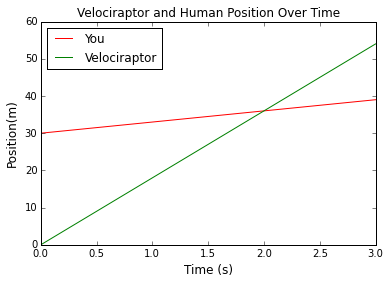
\includegraphics[scale=.6]{graph1.png}

The graph gives an accurate visual representation of the respective paths to set up part two.


\section{Part Two}
This section asks the students to find the exact position where the velociraptor catches up to you, the point of intersection on the graph, without using basic algebra. To approach this problem, I used a loop for a range of values, i, zero to one thousand because there are one thousand points in all of the lists. I then used an if statement to check if the positions of the human, x[i], and the velociraptor, v[i], are equal at a certain time, t[i]. When they are equal, a statement was printed that included the human position, x[i], and the time, t[i]. When the code is run, it returns that the velociraptor catches up to the human at thirty six meters in two seconds.
\section{Part Three}
Section three requires the student to find the point at which the velociraptor is one meter behind them and then graph the paths again with an arrow pointing to the spot. First, I created another for loop with the same approach as part two. However, I used an if statement to find the point when the human position minus the velociraptor position is less than or equal to one, $x[i]-v[i]<=1$. I included the less than symbol because the values are very specific due to the small time intervals and may not be totally equal at any of the given times. If the values at any i make this statement true, then a statement is printed giving the human position, x[i], and the time, t[i]. These values turn out to be 35.802 meters and 1.933 seconds. I also included a break statement after this statement because multiple positions could make the if statement true. I only wanted the first point at which the statement is true.

Next, I recreated the graph from part one using the same code but I added a plot.arrow function with six arguments. The values that the function takes in the x position and y position of the arrow's point of origin, the x length and y length of the arrow tail and the length and width of the arrow head. The x position of the arrow is the time given by the for loop, 1.933 seconds. The y position is based on the y length and arrow head length as well. I wanted my arrow to have a y length of 10.0 meters on the graph and a head length of three meters so I chose for the arrow to start at twenty two meters so it would fall just below the point at 35.802 meters. The x length of the arrow is zero so it will point straight up. I chose the head width to be .1 units just because I liked the way it looks. The graph and arrow are shown below.

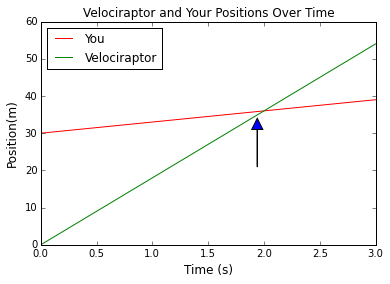
\includegraphics[scale=.6]{graph2.png}


\section{Part Four}
In section four, the student is supposed to find the percent chance of survival when the velociraptor starts trying to bite you one meter behind you. The velociraptor has a twenty percent chance of biting you the first time. If he succeeds, you're dead. If he doesn't he gets frustrated. The second attempt, he only has a fifteen percent chance of catching you. If he misses again, he only has a seven percent chance of biting you. If he misses on this chance, he doesn't try again.

To approach this problem, I created a function called death that doesn't take in any arguments. The function creates one hundred random points between one and one hundred for each of three variables called first, second and third. It then takes these lists of values and runs them through a series of conditional statements. First, if the values in first are less than or equal to twenty, then the function should return "Got ya!" Then, if the values in second are less than or equal to fifteen, the function will return "Dinner time!" Next, if the values of third are less than or equal to seven, the function will return "Finally!" If they functions do not do any of the following, the function will return "You escaped!"

The next thing I did was initialize two variable called escape as zero and created a variable, n, as the number of times you want the function to run. Then, I added a for loop that runs for a range of zero to n. It sets a variable $oh_no$ equal to the death function. Inside the loop, if $oh_no$ equals "Gosh darn it!", the value the function returns if you escape, then it adds one to escape.

Outside of the loop, I created another variable, chances, and set it equal to the value of escape divided by the float of n multiplied by one hundred, to create a percent. The code then prints the value of chances, the percent chance of survival, approximately 61.0%.
\\
\\
\section{Conclusion}
This analysis of the situation described offers a somewhat hopeful chance of escape. You have a better chance of escaping the velociraptor than you do of flipping a head on a coin. However, you would never be able to outrun him and you still have a high chance of meeting "a gruesome demise by the hand of God" in the words of Daniel Edwin Finnegan.

\end{document}
